\documentclass[a4paper,12pt]{article}
\usepackage{docsTemplate}
\usepackage{array}
\usepackage{longtable}
\usepackage{float}
\usepackage[official]{eurosym}
\usepackage{pgf-pie}
\usepackage{makecell}
\usepackage{xltabular}
\usepackage{amsmath}
\usepackage{caption}
\setTitle{Specifica Tecnica}
\setAuthors{Mattia Oliva Medin \\ & Francesco Balestro \\ & Bianca Zaghetto}
\setVerificators{Nenad Radulovic \\ & Filippo Compagno \\ & Francesco Balestro \\ & Bianca Zaghetto}
\setApprovation{}
\setVersion{0.4}
\setType{Esterno}
\setDestination{Team Three Technologies \\ & Prof. Tullio Vardanega \\ & Prof. Riccardo Cardin \\ & Sanmarco Informatica SpA}

\begin{document}
    \include{docTitlepage}

    \section*{Registro delle modifiche} {
        \begin{table}[h!]
            \rowcolors{2}{lightgray}{white}
                \begin{tabularx}{\textwidth}{|l|l|l|l|L|L|}
                \hline
                \textbf{Vers.} & \textbf{Data} & \textbf{Autore} & \textbf{Ruolo} & \textbf{Verifica} & \textbf{Oggetto} \\
                \hline
                \textbf{0.4} & 22/04/26 & Francesco Balestro & Responsabile & Bianca Zaghetto & Prima stesura Architetture e aggiornamento sezione "Tecnologie" \\
                \hline
                \textbf{0.3} & 14/04/26 & Bianca Zaghetto & Programmatore & Francesco Balestro & Riferimenti normativi \\
                \hline
                \textbf{0.2} & 13/04/26 & Francesco Balestro & Verificatore & Filippo Compagno & Sezione "Scopo del documento" e "Tecnologie" \\
                \hline
                \textbf{0.1} & 11/04/26 & Mattia Oliva Medin & Programmatore & Nenad Radulovic & Prima stesura \\
                \hline
            \end{tabularx}
        \end{table}
    }
    \newpage
    
    \tableofcontents
    \newpage

    \listoffigures
    \newpage
    
    \listoftables
    \newpage

    \section{Introduzione} {
        \subsection{Scopo del documento} {        
            Il presente documento ha lo scopo di descrivere in maniera approfondita l’architettura del prodotto software, offrendo una rappresentazione chiara, organizzata e completa delle sue componenti, delle modalità con cui interagiscono e della loro distribuzione all’interno del sistema.\\
            \\
            La Specifica Tecnica costituisce un riferimento fondamentale per le attività di progettazione e sviluppo del prodotto, introducendo evoluzioni e miglioramenti volti a rafforzarne la solidità architetturale rispetto al PoC.\\
            \\
            In particolare, questo documento si propone di:
            \begin{itemize}
                \item Definire l’architettura logica del sistema, descrivendo le componenti principali, le rispettive responsabilità e le relazioni tra esse;
                \item Illustrare l’architettura di deployment, specificando come le diverse componenti vengono distribuite nell’ambiente di esecuzione;
                \item Presentare i design pattern architetturali adottati, mettendo in evidenza le scelte progettuali legate alle tecnologie utilizzate;
                \item Fornire ulteriori dettagli progettuali utili a valorizzare le decisioni architetturali e a facilitare la comprensione e la manutenzione del sistema.
            \end{itemize}
        }

        \subsection{Glossario} {
            Si rimanda al documento Glossario per chiarire i termini nel dominio del progetto che possono risultare ambigui o di difficile comprensione. I vocaboli presenti nel glossario sono stati segnalati seguendo la notazione:
            \begin{center}
                parola\textsubscript{G}
            \end{center}
        }
        
        \subsection{Riferimenti} {
            \subsubsection{Riferimenti normativi} {
                \begin{itemize}
                    \item \textit{Norme di progetto v1.0}
                    \begin{itemize}
                        \item \url{https://team-three-technologies.github.io/Documenti/2%20-%20PB/Documenti%20Interni/Norme_di_Progetto_v1_0.pdf}
                        \item[] (Ultimo accesso: 2026/04/11)
                    \end{itemize}
                    \item Capitolato C3
                    \begin{itemize}
                        \item \url{https://www.math.unipd.it/~tullio/IS-1/2025/Progetto/C3.pdf}
                        \item[] (Ultimo accesso: 2026/01/11)
                    \end{itemize}
                    \item Regolamento del Progetto Didattico
                    \begin{itemize}
                        \item \url{https://www.math.unipd.it/~tullio/IS-1/2025/Dispense/PD1.pdf}
                        \item[] (Ultimo accesso: 2026/04/05)
                    \end{itemize}
                \end{itemize}
            }
            \subsubsection{Riferimenti informativi} {
                \begin{itemize}
                    \item \textit{Glossario v0.5}
                    \begin{itemize}
                        \item \url{https://team-three-technologies.github.io/Documenti/1%20-%20RTB/Documenti%20interni/Glossario_v0_5.pdf}
                        \item[] (Ultimo accesso: 2026/MM/DD)
                    \end{itemize}
                \end{itemize}
            }
        }
    }

    \section{Tecnologie} {
        Il progetto è stato realizzato adottando un insieme di tecnologie consolidate e complementari, selezionate per garantire semplicità di sviluppo, portabilità e facilità di manutenzione, in linea con un’architettura di tipo monolitico.\\
        \\
        La soluzione prevede un’applicazione desktop sviluppata utilizzando Angular per la gestione dell’interfaccia utente, integrata con Electron per la creazione del pacchetto eseguibile e per l’esecuzione in ambiente desktop. La comunicazione tra le componenti avviene tramite meccanismi di Inter-Process Communication (IPC) messi a disposizione da Electron, consentendo un’interazione strutturata ed efficiente tra le diverse parti dell’applicazione.\\
        \\
        Per la gestione della persistenza dei dati è stato adottato SQLite, scelto per la sua leggerezza, semplicità di integrazione e adeguatezza a contesti applicativi locali. In particolare, il database viene utilizzato per memorizzare e gestire i dati relativi al DIP, permettendone la consultazione e la visualizzazione all’interno dell’applicazione.\\
        \\
        Le tecnologie adottate sono state classificate in funzione del loro ruolo architetturale all’interno del sistema, includendo linguaggi di programmazione, framework per lo sviluppo dell’interfaccia utente, framework e runtime per l’esecuzione e il packaging dell’applicazione desktop, meccanismi di comunicazione tra componenti e sistemi di persistenza dei dati.\\
        \\
        Di seguito vengono descritte nel dettaglio le tecnologie adottate, evidenziandone le caratteristiche principali.

        \subsection{Linguaggi di Programmazione}
        \begin{table}[H]
            \captionsetup{skip=10pt}
            \caption{Linguaggi di Programmazione}
            \rowcolors{1}{lightgray}{white}
            \begin{tabular}{|>{\centering\arraybackslash}m{0.20\linewidth}|>{\centering\arraybackslash}m{0.10\linewidth}|>{\centering\arraybackslash}m{0.62\linewidth}|}
                \hline
                \textbf{Tecnologia} & \textbf{Versione} & \textbf{Descrizione} \\
                \hline
                \textbf{TypeScript} & 5.9.3 & TypeScript è un linguaggio di programmazione tipizzato basato su JavaScript, utilizzato per migliorare la qualità del codice grazie alla tipizzazione statica e al supporto per lo sviluppo di applicazioni scalabili e manutenibili. \\
                \hline
            \end{tabular}
        \end{table}

        \subsection{Framework per lo sviluppo dell'interfaccia utente}
        \begin{table}[H]
            \captionsetup{skip=10pt}
            \caption{Framework per lo sviluppo dell'interfaccia utente}
            \rowcolors{1}{lightgray}{white}
            \begin{tabular}{|>{\centering\arraybackslash}m{0.20\linewidth}|>{\centering\arraybackslash}m{0.10\linewidth}|>{\centering\arraybackslash}m{0.62\linewidth}|}
                \hline
                \textbf{Tecnologia} & \textbf{Versione} & \textbf{Descrizione} \\
                \hline
                \textbf{Angular} & 21.2.0 & Angular è un framework frontend basato su TypeScript, utilizzato per la realizzazione di applicazioni web strutturate e modulari tramite un’architettura a componenti. \\
                \hline
            \end{tabular}
        \end{table}

        \subsection{Framework e runtime di esecuzione desktop}
        \begin{table}[H]
            \captionsetup{skip=10pt}
            \caption{Framework e runtime di esecuzione desktop}
            \rowcolors{1}{lightgray}{white}
            \begin{tabular}{|>{\centering\arraybackslash}m{0.20\linewidth}|>{\centering\arraybackslash}m{0.10\linewidth}|>{\centering\arraybackslash}m{0.62\linewidth}|}
                \hline
                \textbf{Tecnologia} & \textbf{Versione} & \textbf{Descrizione} \\
                \hline
                \textbf{Electron} & 40.8.2 & Electron è un framework per lo sviluppo di applicazioni desktop multipiattaforma basato su tecnologie web, che integra un runtime basato su Chromium e Node.js e fornisce strumenti per il packaging e l’esecuzione dell’applicazione. \\
                \hline
            \end{tabular}
        \end{table}

        \subsection{Librerie}
        \begin{table}[H]
            \captionsetup{skip=10pt}
            \caption{Librerie}
            \rowcolors{1}{lightgray}{white}
            \begin{tabular}{|>{\centering\arraybackslash}m{0.20\linewidth}|>{\centering\arraybackslash}m{0.10\linewidth}|>{\centering\arraybackslash}m{0.62\linewidth}|}
                \hline
                \textbf{Tecnologia} & \textbf{Versione} & \textbf{Descrizione} \\
                \hline
                \textbf{ngx-doc-viewer} & 21.0.5 & Libreria Angular per la visualizzazione di documenti direttamente nel browser tramite viewer integrati. \\
                \hline
                \textbf{better-sqlite3} & 12.6.2 & Libreria per Node.js che fornisce un’interfaccia sincrona ed efficiente per l’utilizzo di database SQLite, integrando direttamente il motore SQLite e semplificando l’esecuzione di query e la gestione dei dati. \\
                \hline
                \textbf{fast-xml-parser} & 5.5.9 & Libreria JavaScript veloce per il parsing e la conversione di file XML in oggetti JavaScript, e viceversa. \\
                \hline
                \textbf{tsyringe} & 4.10.0 & Libreria di dependency injection per TypeScript che facilita la gestione delle dipendenze e l’inversione del controllo. \\
                \hline
            \end{tabular}
        \end{table}

        \subsection{Strumenti di sviluppo}
        \begin{table}[H]
            \captionsetup{skip=10pt}
            \caption{Strumenti di sviluppo}
            \rowcolors{1}{lightgray}{white}
            \begin{tabular}{|>{\centering\arraybackslash}m{0.20\linewidth}|>{\centering\arraybackslash}m{0.10\linewidth}|>{\centering\arraybackslash}m{0.62\linewidth}|}
                \hline
                \textbf{Tecnologia} & \textbf{Versione} & \textbf{Descrizione} \\
                \hline
                \textbf{prettier} & 3.8.1 & Prettier è un formatter automatico di codice che garantisce uno stile consistente e leggibile in diversi linguaggi. \\
                \hline
                \textbf{electron-builder} & 26.8.1 & Strumento per il packaging e la distribuzione di applicazioni Electron in eseguibili per diverse piattaforme. \\
                \hline
            \end{tabular}
        \end{table}

        \subsection{Tecnologie per analisi dinamica}
        \begin{table}[H]
            \captionsetup{skip=10pt}
            \caption{Tecnologie per analisi dinamica}
            \rowcolors{1}{lightgray}{white}
            \begin{tabular}{|>{\centering\arraybackslash}m{0.20\linewidth}|>{\centering\arraybackslash}m{0.10\linewidth}|>{\centering\arraybackslash}m{0.62\linewidth}|}
                \hline
                \textbf{Tecnologia} & \textbf{Versione} & \textbf{Descrizione} \\
                \hline
                \textbf{vitest} & 4.0.8 & Vitest è un framework di testing veloce per progetti JavaScript/TypeScript, progettato per integrarsi con Vite e supportare test unitari e di integrazione. \\
                \hline
                \textbf{@vitest/coverage-v8} & 4.0.8 & @vitest/coverage-v8 è un plugin per Vitest che utilizza il motore V8 per generare report di code coverage durante l’esecuzione dei test. \\
                \hline
            \end{tabular}
        \end{table}
    }

    \section{Architettura} {
        \subsection{Architettura logica} {
            Il sistema è progettato seguendo un’\textbf{architettura layered}, che organizza l’applicazione in livelli distinti con responsabilità ben definite, al fine di garantire una chiara separazione delle competenze, una maggiore manutenibilità e una migliore scalabilità logica del sistema.\\
            \\
            In questo modello architetturale, ogni livello espone servizi ben definiti verso il livello superiore e interagisce esclusivamente con quelli adiacenti, riducendo l’accoppiamento tra le componenti. Questa struttura consente di isolare la logica di presentazione, la logica applicativa e la gestione dei dati, facilitando l’evoluzione indipendente delle singole parti del sistema.\\
            \\
            L’applicazione è organizzata in tre livelli principali: \textit{presentation layer}, \textit{application layer} e \textit{data layer}, ciascuno con un ruolo ben definito all’interno del sistema.
            \begin{itemize}
                \item Il \textbf{presentation layer} è responsabile dell’interfaccia utente e della visualizzazione dei contenuti del DIP (Dissemination Information Package). È implementato tramite \textit{Angular} e gestisce il rendering delle viste, l’interazione con l’utente e la presentazione dei documenti e dei metadati.
                \item L'\textbf{application layer} contiene la logica applicativa e coordina le operazioni tra interfaccia utente e accesso ai dati. È integrato nel contesto di \textit{Electron} e si occupa della gestione del flusso applicativo, della comunicazione tra processi tramite IPC e dell’orchestrazione delle operazioni sul DIP
                \item Il \textbf{data layer} gestisce la persistenza e l’accesso ai dati contenuti nel pacchetto DIP. Utilizza \textit{better-sqlite3} per l’interazione con il database locale, permettendo l’esecuzione di query sui metadati e la gestione strutturata delle informazioni archivistiche.\\
            \end{itemize}
            La comunicazione tra i diversi livelli, in particolare tra presentation layer e application layer, avviene attraverso meccanismi di IPC forniti nativamente da Electron, che permettono un’interazione controllata tra i processi mantenendo una separazione tra interfaccia utente e logica applicativa.
        }
        
        \subsection{Architettura di deployment} {
            L’architettura di deployment del sistema è di tipo \textbf{monolitico}, in quanto l’applicazione viene distribuita come un’unica unità software autocontenuta. Tutte le componenti necessarie al funzionamento del sistema, incluse le dipendenze e le risorse applicative, sono incluse all’interno dello stesso pacchetto installabile.\\
            \\
            Questa scelta consente di semplificare il processo di installazione e configurazione per l’utente finale, eliminando la necessità di servizi esterni o di componenti distribuiti. L’applicazione può quindi essere eseguita in locale in modo indipendente, garantendo portabilità e coerenza dell’ambiente di esecuzione.\\
            \\
            Il packaging e la distribuzione dell’applicazione sono gestiti tramite \textit{electron-builder}, uno strumento specifico per applicazioni \textit{Electron}, che consente la creazione di eseguibili per le principali piattaforme desktop. Questo processo permette di ottenere un unico installer che incapsula l’intero sistema e tutte le sue dipendenze.
        }

        \subsection{Design pattern} {
            \subsubsection{Dependency injection} {
                
            }
        }
    }

    \section{Stato dei requisiti funzionali} {
        \subsection{Stato per requisito} {
            \rowcolors{2}{lightgray}{white}
            \begin{longtable}{|>{\centering\arraybackslash}m{0.15\textwidth}|>{\centering\arraybackslash}m{0.5\textwidth}|>{\centering\arraybackslash}m{0.2\textwidth}|}
                \caption{Requisiti Funzionali} \\
                
                \hline
                \rowcolor{lightgray}
                \textbf{Codice} & \textbf{Descrizione} & \textbf{Stato} \\
                \hline
                \endfirsthead
                
                \hline
                \rowcolor{lightgray}
                \textbf{Codice} & \textbf{Descrizione} & \textbf{Stato} \\
                \hline
                \endhead
                
                \textbf{R1-F-Ob} & L'utente deve poter caricare un DIP nel sistema avviando l'applicazione all'interno del DIP estratto & 
                Soddisfatto \\
                \hline
                \textbf{R2-F-Ob} & L'utente deve ricevere un messaggio di errore se il caricamento del DIP non avviene correttamente & 
                Soddisfatto \\
                \hline
                \textbf{R3-F-Ob} & L'utente deve poter visualizzare il contenuto e le informazioni del DIP & Soddisfatto \\ 
                \hline
                \textbf{R4-F-Ob} & L'utente deve poter visualizzare i singoli documenti, e la lista dei loro allegati, contenuti nel DIP & 
                Soddisfatto \\ 
                \hline
                \textbf{R5-F-Ob} & L'utente deve poter visualizzare i singoli allegati di un documento & Soddisfatto \\ 
                \hline
                \textbf{R6-F-Ob} & L'utente deve poter visualizzare i dettagli di un documento & Soddisfatto \\ 
                \hline
                \textbf{R7-F-Ob} & L'utente deve poter visualizzare la tipologia documentale di un documento & Soddisfatto \\
                \hline
                \textbf{R8-F-Ob} & L'utente deve poter visualizzare il numero di un documento & Soddisfatto \\
                \hline
                \textbf{R9-F-Ob} & L'utente deve poter visualizzare il codice registro di un documento & Soddisfatto \\
                \hline
                \textbf{R10-F-Ob} & L'utente deve poter visualizzare la lista dei soggetti coinvolti in un documento & Soddisfatto \\ 
                \hline
                \textbf{R11-F-Ob} & L'utente deve poter visualizzare il singolo soggetto coinvolto in un documento & 
                Soddisfatto \\ 
                \hline
                \textbf{R12-F-Ob} & L'utente deve poter visualizzare il ruolo di un soggetto coinvolto in un documento & Soddisfatto \\ 
                \hline
                \textbf{R13-F-Ob} & L'utente deve poter visualizzare l'oggetto di un documento & Soddisfatto \\ 
                \hline
                \textbf{R14-F-Ob} & L'utente deve poter visualizzare il tipo aggregazione di un documento & Soddisfatto \\ 
                \hline
                \textbf{R15-F-Ob} & L'utente deve poter visualizzare le informazioni di conservazione di un DIP & Soddisfatto \\ 
                \hline
                \textbf{R16-F-Ob} & Il Sistema deve eseguire i controlli sulla validità e lo stato del processo di conservazione & Soddisfatto \\ 
                \hline
                \textbf{R17-F-De} & L'utente deve poter impostare il criterio "Impronta crittografica" per cercare un documento & 
                Soddisfatto \\ 
                \hline
                \textbf{R18-F-Ob} & L'utente deve poter impostare il criterio "Identificativo documento" per cercare un documento & 
                Soddisfatto \\ 
                \hline
                \textbf{R19-F-De} & L'utente deve poter impostare il criterio "Modalità di formazione" per cercare un documento & 
                Soddisfatto \\ 
                \hline
                \textbf{R20-F-Ob} & L'utente deve poter impostare il criterio "Tipologia documentale" per cercare un documento & 
                Soddisfatto \\ 
                \hline
                \textbf{R21-F-De} & L'utente deve poter impostare il criterio "Tipologia di flusso" per cercare un documento & 
                Soddisfatto \\ 
                \hline
                \textbf{R22-F-De} & L'utente deve poter impostare il criterio "Tipo registro" per cercare un documento & 
                Soddisfatto \\
                \hline
                \textbf{R23-F-Ob} & L'utente deve poter impostare il criterio "Data registrazione" per cercare un documento & 
                Soddisfatto \\ 
                \hline
                \textbf{R24-F-Ob} & L'utente deve poter impostare il criterio "Ora registrazione" per cercare un documento & 
                Soddisfatto \\ 
                \hline
                \textbf{R25-F-Ob} & L'utente deve poter impostare il criterio "Numero documento" per cercare un documento & 
                Soddisfatto \\ 
                \hline
                \textbf{R26-F-Ob} & L'utente deve poter impostare il criterio "Codice registro" per cercare un documento & 
                Soddisfatto \\ 
                \hline
                \textbf{R27-F-Ob} & L'utente deve poter impostare il criterio "Ruolo" per cercare un documento & 
                Soddisfatto \\ 
                \hline
                \textbf{R28-F-Ob} & L'utente deve poter impostare il criterio "Tipo soggetto" per cercare un documento & 
                Soddisfatto \\ 
                \hline
                \textbf{R29-F-Ob} & L'utente deve poter impostare il criterio "Cognome" per cercare un documento & 
                Soddisfatto \\ 
                \hline
                \textbf{R30-F-Ob} & L'utente deve poter impostare il criterio "Nome" per cercare un documento & 
                Soddisfatto \\ 
                \hline
                \textbf{R31-F-Ob} & L'utente deve poter impostare il criterio "Codice Fiscale" per cercare un documento & 
                Soddisfatto \\ 
                \hline
                \textbf{R32-F-De} & L'utente deve poter impostare il criterio "Indirizzo digitale" per cercare un documento & 
                Soddisfatto \\ 
                \hline
                \textbf{R33-F-De} & L'utente deve poter impostare il criterio "Denominazione organizzazione" per cercare un documento & 
                Soddisfatto \\ 
                \hline
                \textbf{R34-F-De} & L'utente deve poter impostare il criterio "Partita IVA" per cercare un documento & 
                Soddisfatto \\ 
                \hline
                \textbf{R35-F-De} & L'utente deve poter impostare il criterio "Denominazione ufficio" per cercare un documento & 
                Soddisfatto \\ 
                \hline
                \textbf{R36-F-De} & L'utente deve poter impostare il criterio "Denominazione amministrazione" per cercare un documento & 
                Soddisfatto \\
                \hline
                \textbf{R37-F-De} & L'utente deve poter impostare il criterio "Codice IPA" per cercare un documento & 
                Soddisfatto \\
                \hline
                \textbf{R38-F-De} & L'utente deve poter impostare il criterio "Denominazione amministrazione AOO" per cercare un documento & 
                Soddisfatto \\
                \hline
                \textbf{R39-F-De} & L'utente deve poter impostare il criterio "Codice IPA AOO" per cercare un documento & 
                Soddisfatto \\
                \hline
                \textbf{R40-F-De} & L'utente deve poter impostare il criterio "Denominazione amministrazione UOR" per cercare un documento & 
                Soddisfatto \\
                \hline
                \textbf{R41-F-De} & L'utente deve poter impostare il criterio "Codice IPA UOR" per cercare un documento & 
                Soddisfatto \\
                \hline
                \textbf{R42-F-De} & L'utente deve poter impostare il criterio "Denominazione sistema" per cercare un documento & 
                Soddisfatto \\ 
                \hline
                \textbf{R43-F-Ob} & L'utente deve poter impostare il criterio "Oggetto" per cercare un documento & 
                Soddisfatto \\ 
                \hline
                \textbf{R44-F-De} & L'utente deve poter impostare il criterio "Parola chiave" per cercare un documento & 
                Soddisfatto \\ 
                \hline
                \textbf{R45-F-De} & L'utente deve poter impostare il criterio "Numero allegati" per cercare un documento & 
                Soddisfatto \\ 
                \hline
                \textbf{R46-F-De} & L'utente deve poter impostare il criterio "Impronta crittografica allegato" per cercare un documento & 
                Soddisfatto \\ 
                \hline
                \textbf{R47-F-De} & L'utente deve poter impostare il criterio "Identificativo allegato" per cercare un documento & 
                Soddisfatto \\ 
                \hline
                \textbf{R48-F-De} & L'utente deve poter impostare il criterio "Descrizione allegato" per cercare un documento & 
                Soddisfatto \\ 
                \hline
                \textbf{R49-F-De} & L'utente deve poter impostare il criterio "Indice di classificazione" per cercare un documento & 
                Soddisfatto \\ 
                \hline
                \textbf{R50-F-De} & L'utente deve poter impostare il criterio "Descrizione dell'indice di classificazione" per cercare un documento & 
                Soddisfatto \\ 
                \hline
                \textbf{R51-F-De} & L'utente deve poter impostare il criterio "Piano di classificazione" per cercare un documento & 
                Soddisfatto \\ 
                \hline
                \textbf{R52-F-De} & L'utente deve poter impostare il criterio "Riservato" per cercare un documento & 
                Soddisfatto \\ 
                \hline
                \textbf{R53-F-Ob} & L'utente deve poter impostare il criterio "Formato" per cercare un documento & 
                Soddisfatto \\ 
                \hline
                \textbf{R54-F-De} & L'utente deve poter impostare il criterio "Nome prodotto software" per cercare un documento & 
                Soddisfatto \\ 
                \hline
                \textbf{R55-F-De} & L'utente deve poter impostare il criterio "Versione prodotto software" per cercare un documento & 
                Soddisfatto \\ 
                \hline
                \textbf{R56-F-De} & L'utente deve poter impostare il criterio "Produttore software" per cercare un documento & 
                Soddisfatto \\ 
                \hline
                \textbf{R57-F-De} & L'utente deve poter impostare il criterio "Firmato digitalmente" per cercare un documento & 
                Soddisfatto \\ 
                \hline
                \textbf{R58-F-De} & L'utente deve poter impostare il criterio "Sigillato elettronicamente" per cercare un documento & 
                Soddisfatto \\ 
                \hline
                \textbf{R59-F-De} & L'utente deve poter impostare il criterio "Marcatura temporale" per cercare un documento & 
                Soddisfatto \\ 
                \hline
                \textbf{R60-F-De} & L'utente deve poter impostare il criterio "Conformità copie immagine su supporto informatico" per cercare un documento & 
                Soddisfatto \\ 
                \hline
                \textbf{R61-F-Ob} & L'utente deve poter impostare il criterio "Tipo aggregazione" per cercare un documento & 
                Soddisfatto \\ 
                \hline
                \textbf{R62-F-De} & L'utente deve poter impostare il criterio "Identificativo aggregazione" per cercare un documento & 
                Soddisfatto \\ 
                \hline
                \textbf{R63-F-De} & L'utente deve poter impostare il criterio "Tipologia fascicolo" per cercare un documento & 
                Soddisfatto \\ 
                \hline
                \textbf{R64-F-Ob} & L'utente deve poter impostare il criterio "Nome del documento" per cercare un documento & 
                Soddisfatto \\ 
                \hline
                \textbf{R65-F-De} & L'utente deve poter impostare il criterio "Versione del documento" per cercare un documento & 
                Soddisfatto \\ 
                \hline
                \textbf{R66-F-De} & L'utente deve poter impostare il criterio "Tipo modifica" per cercare un documento & 
                Soddisfatto \\ 
                \hline
                \textbf{R67-F-De} & L'utente deve poter impostare il criterio "Data modifica" per cercare un documento & 
                Soddisfatto \\ 
                \hline
                \textbf{R68-F-De} & L'utente deve poter impostare il criterio "Ora modifica" per cercare un documento & 
                Soddisfatto \\ 
                \hline
                \textbf{R69-F-De} & L'utente deve poter impostare il criterio "Tempo di conservazione" per cercare un documento & 
                Soddisfatto \\ 
                \hline
                \textbf{R70-F-De} & L'utente deve poter impostare il criterio "Note" per cercare un documento & 
                Soddisfatto \\ 
                \hline
                \textbf{R71-F-Ob} & L'utente deve poter cercare un documento impostando uno o più criteri di ricerca & 
                Soddisfatto \\ 
                \hline
                \textbf{R72-F-Ob} & L'utente deve poter visualizzare i risultati della ricerca, cioè i documenti che soddisfano i criteri di ricerca impostati & 
                Soddisfatto \\ 
                \hline
                \textbf{R73-F-Ob} & L'utente deve poter visualizzare le informazioni relative ai singoli documenti che rappresentano il risultato della ricerca & 
                Soddisfatto \\ 
                \hline
                \textbf{R74-F-Ob} & L'utente deve ricevere un messaggio informativo se il risultato della ricerca è vuoto, cioè se nessun documento soddisfa i criteri di ricerca impostati & 
                Soddisfatto \\ 
                \hline
                \textbf{R75-F-Ob} & L'utente deve poter visualizzare l'anteprima di un documento selezionato & 
                Soddisfatto \\ 
                \hline
                \textbf{R76-F-Ob} & L'utente deve ricevere un messaggio di avviso sull'eventuale indisponibilità dell'anteprima per un documento selezionato & 
                Soddisfatto \\ 
                \hline
                \textbf{R77-F-Ob} & L'utente deve poter esportare un documento selezionato, scegliendo il percorso dove salvarlo & 
                Soddisfatto \\ 
                \hline
                \textbf{R78-F-Ob} & L'utente deve ricevere un messaggio di errore se l'esportazione fallisce & 
                Soddisfatto \\ 
                \hline
                \textbf{R79-F-Op} & L'utente deve poter configurare la ricerca semantica inserendo una query in linguaggio naturale & 
                Soddisfatto \\ 
                \hline
                \textbf{R80-F-Op} & L'utente deve poter visualizzare il risultato della ricerca semantica configurata & 
                Soddisfatto \\ 
                \hline
                \hline
                \textbf{R80-F-Op} & L'utente deve poter visualizzare il risultato della ricerca semantica configurata & 
                Soddisfatto \\ 
                \hline
                \textbf{R81-F-Op} & L'utente deve poter stampare un documento selezionato & 
                Soddisfatto \\ 
                \hline
                \textbf{R82-F-Ob} & L'utente deve ricevere un messaggio di errore se la stampa fallisce & 
                Soddisfatto \\ 
                \hline
                \textbf{R83-F-Op} & L'utente deve poter verificare la firma digitale di un documento selezionato & 
                Soddisfatto \\ 
                \hline
                \textbf{R84-F-Op} & L'utente deve poter visualizzare il risultato della verifica della firma digitale di un documento & 
                Soddisfatto \\ 
                \hline
            \end{longtable}
        }
        \subsection{Grafici Riassuntivi}
        \begin{figure}[H]
                \centering
                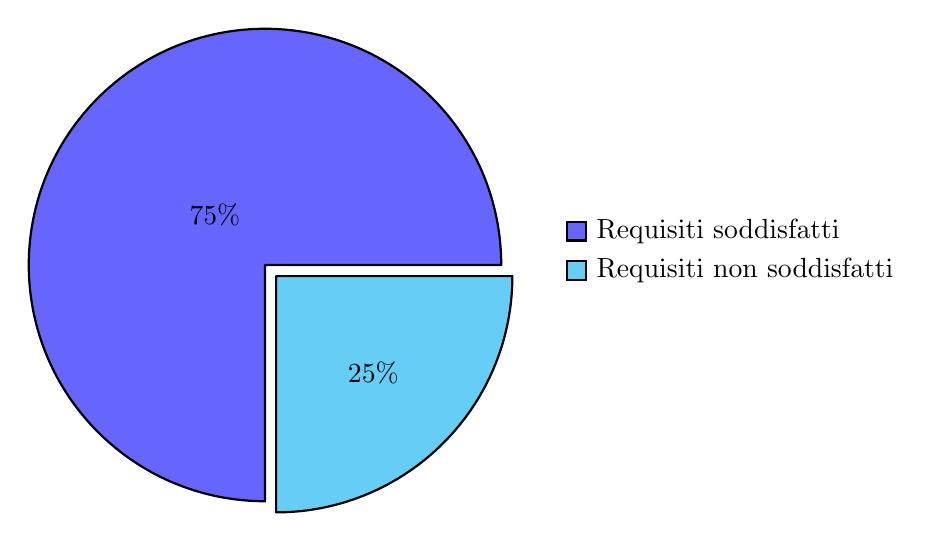
\begin{tikzpicture}
                \pie [explode=0.1, text=legend] { 75/Requisiti soddisfatti, 25/Requisiti non soddisfatti }
                \end{tikzpicture}
                \caption{Percentuale di requisiti funzionali soddisfatti}
        \end{figure}
        \begin{figure}[H]
                \centering
                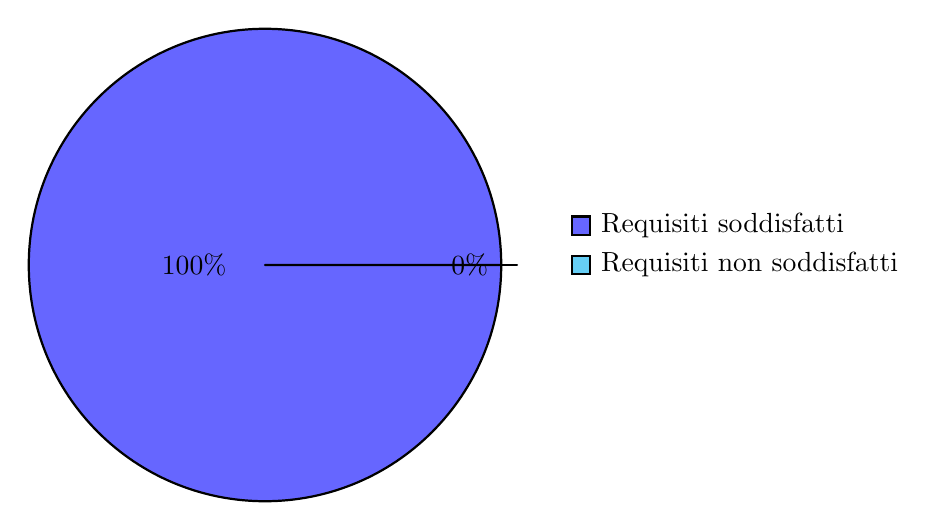
\begin{tikzpicture}
                \pie [explode=0.1, text=legend] { 100/Requisiti soddisfatti, 0/Requisiti non soddisfatti }
                \end{tikzpicture}
                \caption{Percentuale di requisiti funzionali obbligatori soddisfatti}
        \end{figure}
        \begin{figure}[H]
                \centering
                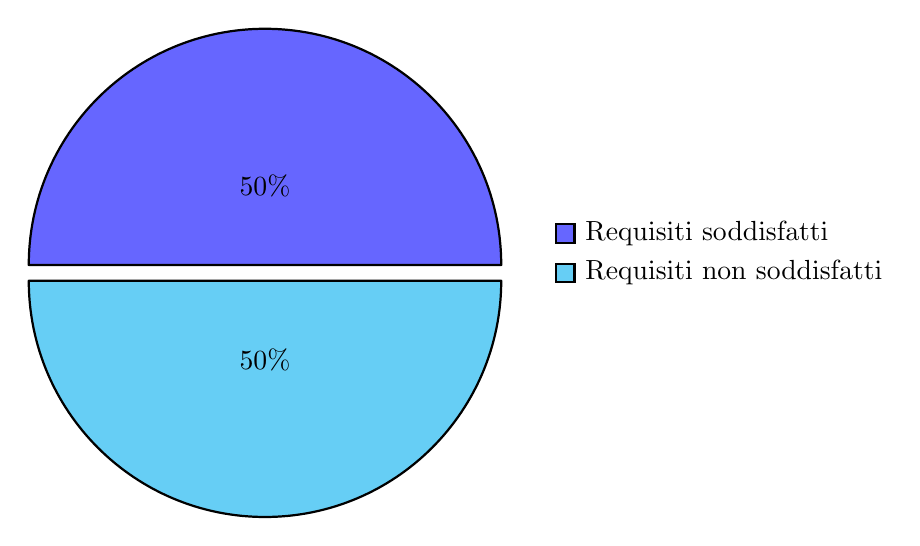
\begin{tikzpicture}
                \pie [explode=0.1, text=legend] { 50/Requisiti soddisfatti, 50/Requisiti non soddisfatti }
                \end{tikzpicture}
                \caption{Percentuale di requisiti funzionali opzionali soddisfatti}
        \end{figure}
        \begin{figure}[H]
                \centering
                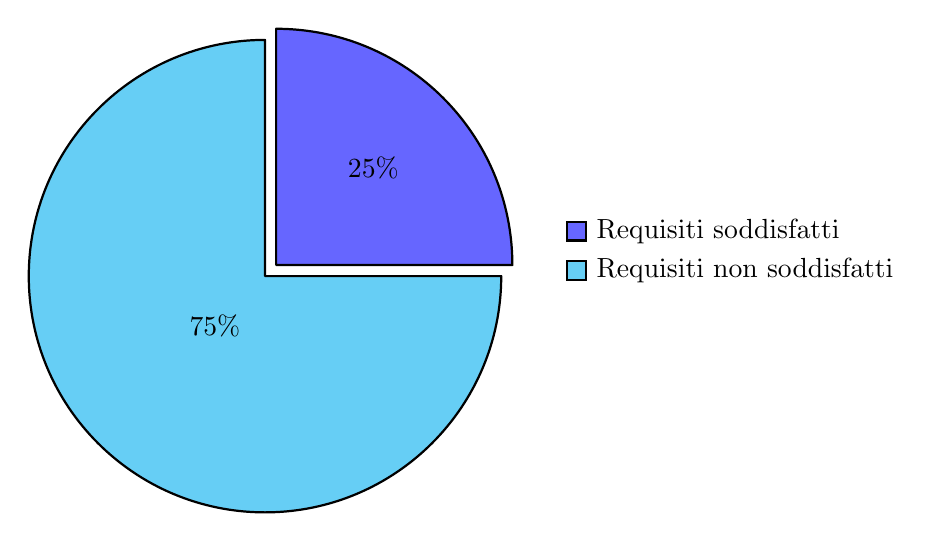
\begin{tikzpicture}
                \pie [explode=0.1, text=legend] { 25/Requisiti soddisfatti, 75/Requisiti non soddisfatti }
                \end{tikzpicture}
                \caption{Percentuale di requisiti funzionali desiderabili soddisfatti}
        \end{figure}
    }
\end{document}
